\documentclass{article}
\usepackage[utf8]{inputenc}
\usepackage{parskip}
\usepackage{amsmath}
\usepackage{wrapfig,floatflt}
\usepackage{natbib}
\usepackage{graphicx}

\title{Mixed layer trapping models}
\author{Jeffrey J. Early and Pete Gaube}
\date{February 2020}

\DeclareMathOperator{\sech}{sech}

\begin{document}

\maketitle

\section{Introduction}

The goal is to create a simple mixed-layer plus geostrophic eddy model which can be used to assess the amount of trapping expected in the surface mixed layer.

The mixed layer models considered will be a damped-slab model, and a few of the other models from \cite{elipot2009-os}.

%%%%%%%%%%%%%%%%%%%%%%%%%%%
%
\subsection{Stratification}
%
%%%%%%%%%%%%%%%%%%%%%%%%%%%


We want to think of this as an equivalent barotropic model for the QG portion---that is, a single baroclinic mode, with no pressure at the bottom boundary. Typical first baroclinic modes in the ocean have an equivalent depth of 80 cm in the ocean. So, we want to maintain the following integral,
\begin{equation}
    80 \textrm{ cm} = \frac{1}{g \pi^2} \left[ \int_{-D}^0 N(z) \, dz \right]^2
\end{equation}{}
when we create our toy density profile.

So let's do the following model: exponential decay in the interior, pycnocline near the surface
\begin{equation}
    N^2(z) = N_0^2 \exp \left[2 \left( \frac{z+D}{L} + \ln \frac{N_b}{N_0} \right)\left( \frac{1-\tanh\left(\frac{z-z_p}{\delta_p}\right)}{2} \right) \right]
\end{equation}{}
where the $\tanh$ function gives us the change to the mixed layer. The whole term is 1 at $z=-D$, and 0 at $z=0$. \textbf{This profile has a mixed layer, but no jump in density crossing the transition layer.} See figure \ref{modes-no-deltarho}

\begin{figure}
\vspace{-30pt}
    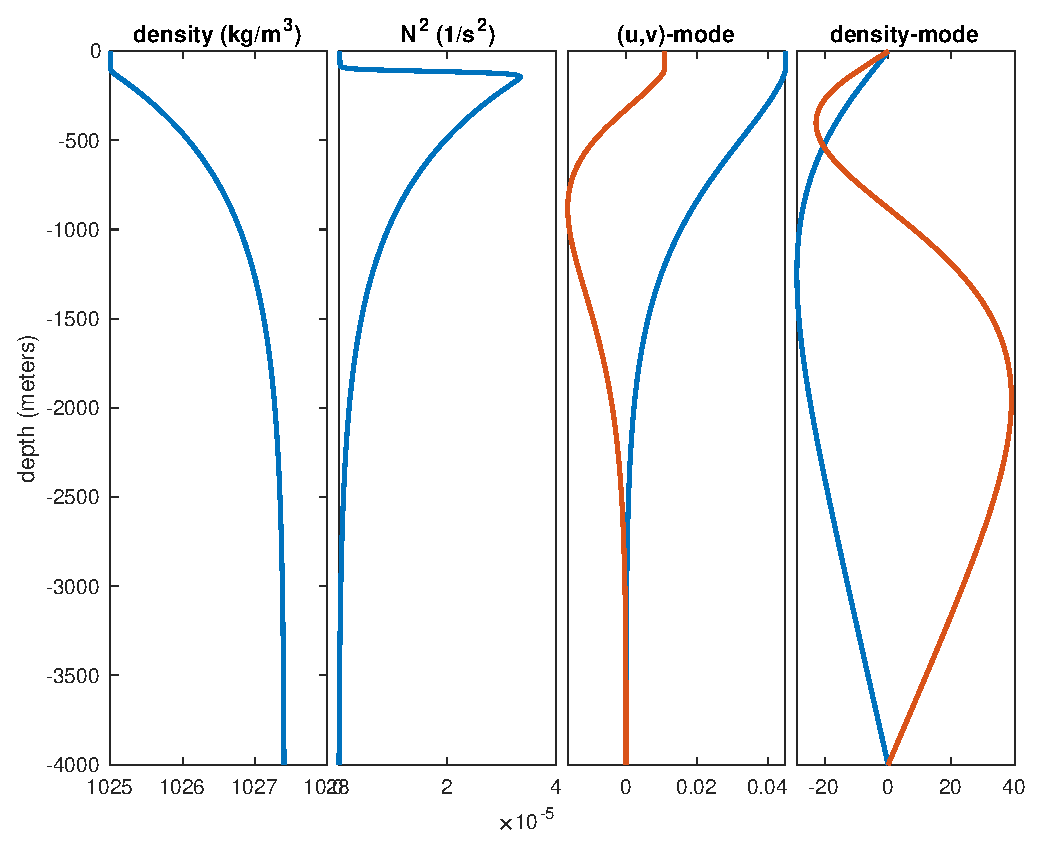
\includegraphics[width=1.0\textwidth]{ModesWithDeltaRho0}
  \caption{Basic stratification profile with \emph{no} density jump after the mixed layer. Interior modes 1 and 2 are shown, blue and red.}
  \label{modes-no-deltarho}
\end{figure}

So now let's add a classic little pycnocline as a $\sech^2(z)$ that we can use to tune the density jump.
\begin{equation}
    N^2(z) = N_0^2 \exp \left[ \left( \frac{z+D}{L} + \ln \frac{N_b}{N_0} \right)\left( 1-\tanh\left(\frac{z-z_p}{\delta_p}\right) \right) \right] + N_\textrm{ml}^2 \sech^2 \left(\frac{z-z_p}{\delta_p}\right)
\end{equation}{}
The value $N^2_ml$ can be set with the required change in density across the jump. Integrating the $\sech^2(z)$ function (to get $\rho$) gives you a $\tanh(z)$ function with amplitude 2. So,
\begin{equation}
    N_\textrm{ml}^2 = \frac{g \Delta \rho }{2 \rho_0 \delta_p}
\end{equation}{}
is the appropriate amplitude to set. Look at Latmix data from the summer time in the Sargasso, and it seems like $\Delta \rho$ can certainly be on the order of 2 $kg/m^3$.
\begin{figure}
\vspace{-30pt}
    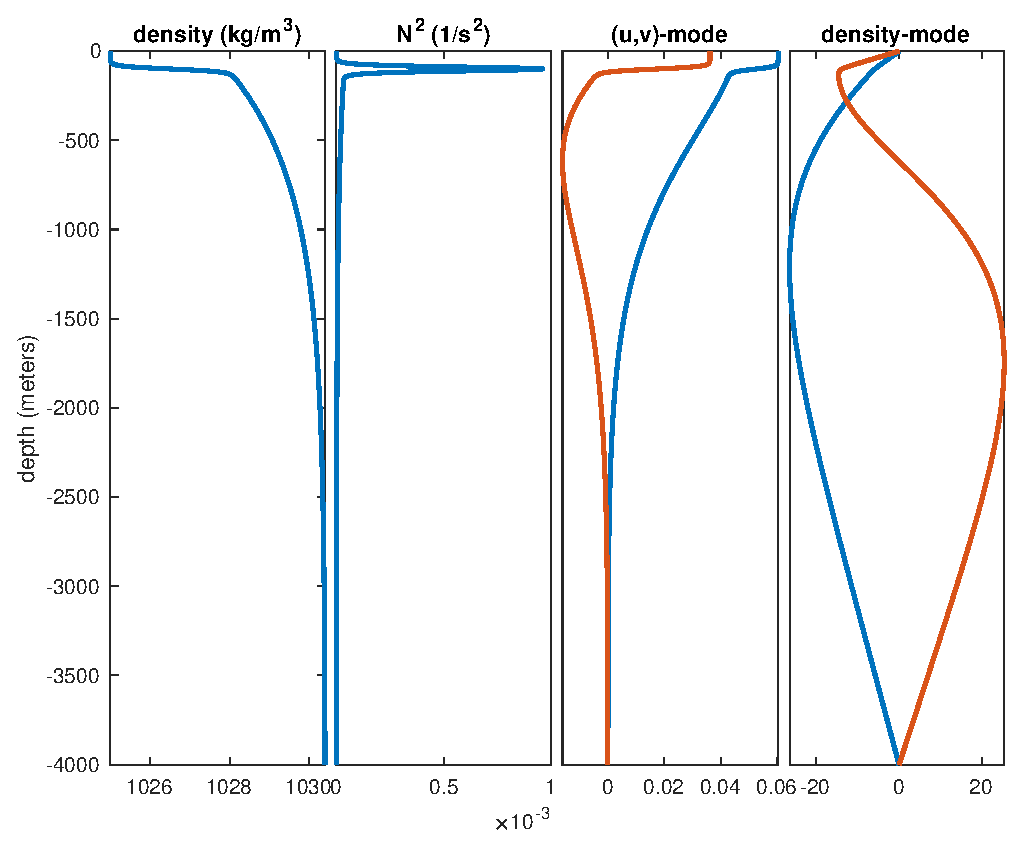
\includegraphics[width=1.0\textwidth]{ModesWithDeltaRho3}
  \caption{Basic stratification profile with a sizeable density jump after the mixed layer. Interior modes 1 and 2 are shown, blue and red.}
  \label{modes-no-deltarho}
\end{figure}

%%%%%%%%%%%%%%%%%%%%%%%%%%%
%
\subsection{Lowest mode comparison}
%
%%%%%%%%%%%%%%%%%%%%%%%%%%%

Now let's check out the 

\begin{figure}
\vspace{-30pt}
    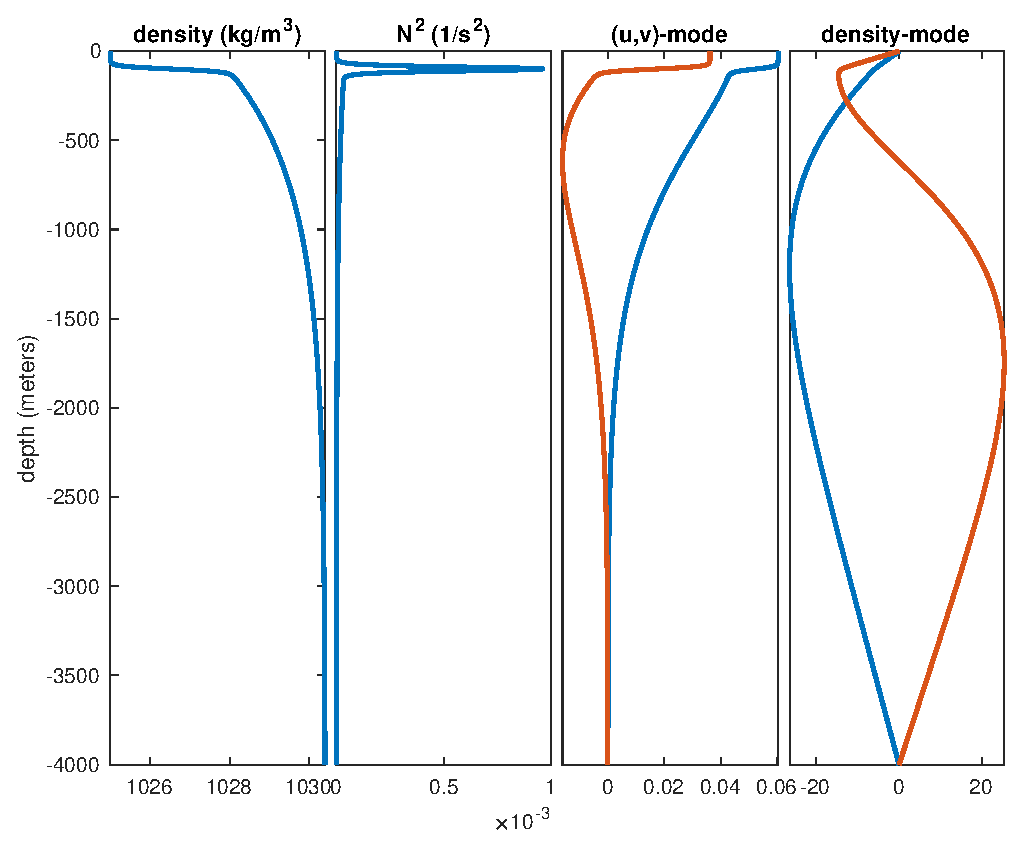
\includegraphics[width=1.0\textwidth]{ModesWithDeltaRho3}
  \caption{Basic stratification profile with a sizeable density jump after the mixed layer. Interior modes 1 and 2 are shown, blue and red.}
  \label{modes-no-deltarho}
\end{figure}

\bibliography{references}

\end{document}
